\chapter{Parser-Modul}

{\color{red} Kurze Einführung (siehe Kapitel zu Core, RISC-V) }

\section{Funktionalität}

Das Parser-Modul liest den gegebenen Assembler-Code, führt alle gegebenen
Compiler-Direktiven aus und generiert für jedes Argument einen Syntax-Baum, der
an die Architektur übergeben wird.  Außerdem reserviert er den über die
Reservierungs- und Definierungsdirektiven festgelegten Speicher.

Somit entspricht der Parser dem Assemblierer.  Die Trennung von Architektur und
Parser wurde vorgenommen, um Code-Duplikation zu vermeiden, die bei
Architekturen mit mehreren Dialekten auftreten könnten (bei X86 z.B. AT\&T- und
Intel-Syntax).

Weiterhin assitiert der Parser mit dem Befehlssatz der Architektur der GUI beim
Syntax-Highlighting.

\section{Umsetzung (Referenzmodul)}

Das Referenzmodul (welches im Rahmen dieses Großpraktikums konstruiert werden
soll) wird als bekannter 2-Pass-Assembler realisiert. Wie die Architektur wird
dieses vorerst auf RISC-V (und hier einen bestimmten Dialekt) ausgelegt und
spezialisiert sein.

\subsection{Entfernen von Kommentaren}

Zuvor werden alle Kommentare entfernt. Dieser Schritt ist nur notwendig, falls
der RISC-V-Assembler mehrzeilige Kommentare unterstützen soll.

\subsection{1. Pass}

Im ersten Schritt wird der rohe Assemblertext gelesen und in Zeilenbereiche
unterteilt, die jeweils einen Befehl mit allen zugehörigen Marken beinhalten.
(alternativ steht momentan zur Diskussion, dass nur die veränderten
Assemblertextteile gelesen und neu analysiert werden, da dies eine bessere
Ausführungsgeschwindigkeit mit sich bringt.  Es würde natürlich bedeuten, dass
alle hier genannten Objekte, Symbole usw. über die Laufzeit des Programmes über
gespeichert werden.)  Diese Befehle werden anschließend in Objekte gepackt (mit
Zeilenintervall und Datei des Auftretens), wobei wir zwischen Direktiven und den
eigentlichen Befehlen unterscheiden.  Besonders bei ersteren wird bereits hier
genauer unterschieden.  Alle Labels und eventuell auch Konstantennamen (die wie
Labels behandelt werden) werden in die Symboltabelle mit ihrem
korrespondierenden (Text-)Wert geschrieben.  Wenn von Core oder GUI gewünscht
(also wenn das Programm gerade nicht läuft), wird hier der Speicher reserviert,
sonst werden nur die entsprechenden Positionen berechnet.  Bei allen Makros wird
Anfang und Ende erfasst und diese in eine separate Makroliste eingetragen.

\subsection{2. Pass}

Wir haben nun eine Befehlsfolge von Objekten. In diesem Schritt werden nun die
Direktiven ausgeführt und die Labels mit ihrem Wert eingesetzt.  Ein Befehl wird
zu einem großen Syntaxbaum umgewandelt. (in Diskussion: Nur aus jedem der
Argumente wird ein Syntaxbaum gebildet. Die Entscheidung steht noch aus) Wegen
möglichen unbekannten Datentypen anderer ISAs usw. wird hier eine Factory für
Knoten vom Architektur-Modul bereitgestellt.  Als Ausgabe dient schließlich eine
Liste von Objekten \emph{ohne} jegliche Direktiven und mit Argumenten als
Syntaxbäumen. Diese wird dann dem Core zur Verfügung gestellt.

\begin{figure}[h!]
  \centering
  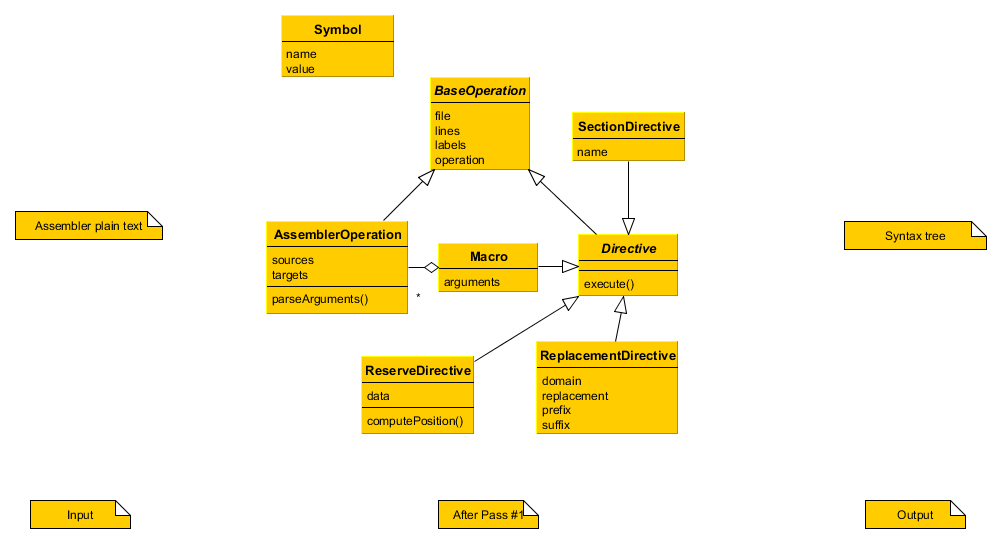
\includegraphics[width=0.8\textwidth]{../parser/figures/process.png}
  \caption{Eine grobe Skizze des geplanten Parsing-Prozesses nach aktuellem Stand.}
\end{figure}

\subsection{Geplante Direktiven-Unterstützung} Unterstützt werden sollen:

\begin{itemize}
\item Makros
\item Speicherreservierungs- und Speicherbelegungs-Direktiven (z.B. resb, dd)
\item Konstantendefinitionen und Aliase (z.B. für Register)
\item Data-/Text-Sektion-Umschaltung
\end{itemize}

\emph{Nicht} unterstützt werden sollen:

\begin{itemize}
\item Bedingte Assemblerkompilierung
\item Komplett freie Textersetzungssysteme (z.B. C-Präprozessor)
\item Inkludieren anderer Assembler-Dateien
\end{itemize} Ebenfalls werden nur einzeilige Kommentare unterstützt werden.

\section{Abhängigkeiten} Der Parser kommuniziert mit allen anderen Modulen
über den Core und ist somit alleine von diesem abhängig.  Die Architektur
erfragt vom Parser die einzelnen assemblierten Zeilen, um diese auszuführen.
Die GUI erhält vom Parser die Fehlermeldungen und stellt die Anfragen, um Code
zu übersetzen.

Eine weitere Funktion des Parsers ist die Bereitstellung von dialektspezifisch
angepassten regulären Ausdrücken, die zum Syntax-Highlighting benutzt werden
können.  Hierzu bekommt der Parser über den Core von der Architektur eine Liste
mit Schlüsselwörtern wie Befehlen, Registernamen und ähnlichem. Der Parser
ergänzt diese dann je nach Dialekt (z.B. Präfixe für Register/Konstanten).  Die
so entstandenen regulären Ausdrücke können nun vom GUI-Modul abgefragt werden.

Wir haben uns dazu entschieden, vorerst die boost::spirit-Bibliothek zu
verwenden, um Ausdrücke zu parsen.  Wir erachten dies als sinnvoll, um das
Projekt in Anbetracht der Stärke des Parser-Teams (zwei Personen) und der
verfügbaren Zeit ordentlich fertigstellen zu können.

\section{Verworfen: Allgemeiner Parser} Im Laufe unserer Entscheidungsfindung
stand auch kurz auf dem Plan, einen allgemeinen Parser mit einem kleinen
dialektabhängigen Modul zu entwerfen.  Dies hätte den Vorteil, dass die
Dialektmodule wesentlich kleiner und einfacher zu programmieren ausgefallen
wären, da die Hauptarbeit ja sowieso der große allgemeine Parser übernimmt.
Jedoch haben wir diese Idee für dieses Großpraktikum verworfen, da hierbei zu
viele Komplikationen entstanden (wie will man fast alle Assemblersprachen
verallgemeinern?).  Sie steht jedoch für spätere Projekte frei, verwendet zu
werden.